% ============================================================
% Procedimiento - SIEMENS (Lab físico)
% Plantilla con descripciones y placeholders de imágenes
% ============================================================

\section{Procedimiento}

\subsection{Siemens}

\subsubsection{Control de ratio de caudal}

\begin{enumerate}[label=\alph*)]
    \item Diseñe un \textbf{controlador de caudal FC11} con el variador de frecuencia \textbf{G120} y el flujómetro \textbf{FT11} utilizando el bloque de instrucción \textbf{PID Compact} con la configuración que se muestra en la tabla. Cree todas las variables necesarias.

    \begin{table}[H]
    \centering
    \renewcommand{\arraystretch}{1.2}
    \setlength{\tabcolsep}{5pt}
    \begin{tabular}{|>{\centering\arraybackslash}m{0.52\linewidth}|>{\centering\arraybackslash}m{0.24\linewidth}|}
    \hline
    \multicolumn{2}{|c|}{\textbf{PID-FC11}} \\ \hline
    \textbf{Tipo de regulación} & Caudal (l/min) \\ \hline
    \textbf{Parámetros de entrada/salida} & \makecell[c]{Input: Input \\ Output: Output} \\ \hline
    \textbf{Límites del valor real} & 0.0 -- 80.0 l/min \\ \hline
    \textbf{Límites del valor de salida} & 0.0 -- 100 \% \\ \hline
    \end{tabular}
    \end{table}

    Se configuró el bloque \textbf{PID Compact} para el controlador FC11 con el tipo de regulación \textit{Caudal (l/min)}, conectando como entrada la lectura del flujómetro FT11 y como salida el comando de velocidad al variador G120. Se establecieron los límites del valor de salida en \textbf{0--100\,\%}, coherentes con el rango operativo del G120, y los límites del valor real en \textbf{0--80 l/min}.

    \begin{figure}[H]
        \centering
        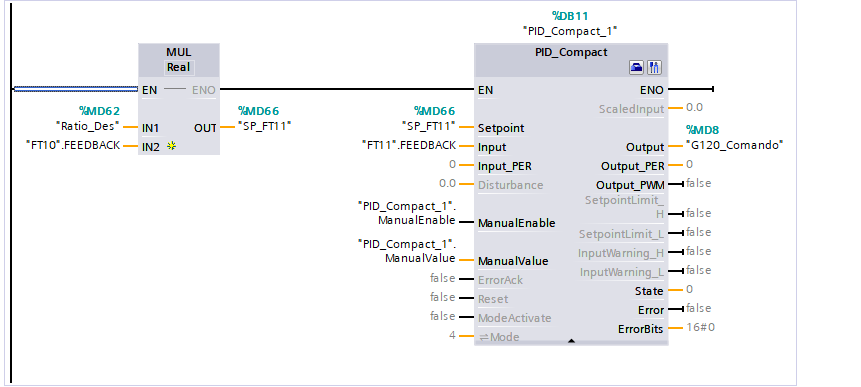
\includegraphics[width=0.85\textwidth]{images/proc_siemens_pid_fc11_config.png}
        \caption{Configuración del bloque PID Compact para el controlador FC11 en TIA Portal.}
        \label{fig:proc_siemens_pid_fc11_config}
    \end{figure}

    \item Diseñe el \textbf{control de ratio de caudal}. Tenga en cuenta que el \textbf{caudal controlado} se mide con \textbf{FT11} y el \textbf{caudal no controlado} se mide con \textbf{FT10}, de modo que el \textbf{Ratio} = \textbf{FT11/FT10}. Utilice las instrucciones \textbf{MUL} para obtener el \textbf{setpoint de caudal para FC11} en función del \textbf{ratio deseado} y el caudal de \textbf{FT10}, \textbf{DIV} para calcular el \textbf{ratio real} y \textbf{SEL} para cambiar entre un \textbf{setpoint manual o de ratio de caudal}.

    Se implementó la lógica del control de ratio en TIA Portal utilizando: una instrucción \textbf{MUL} que multiplica el caudal medido FT10 por el ratio deseado para generar el setpoint de FC11, una instrucción \textbf{DIV} que calcula el ratio real como FT11/FT10, y una instrucción \textbf{SEL} que permite alternar entre un setpoint manual y el setpoint calculado por el ratio.

    \begin{figure}[H]
        \centering
        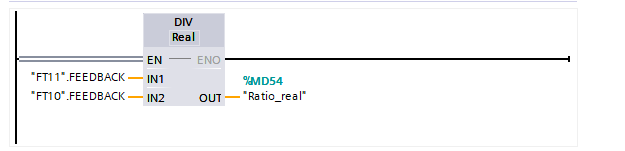
\includegraphics[width=0.95\textwidth]{images/proc_siemens_logica_ratio.png}
        \caption{Lógica del control de ratio implementada en TIA Portal con bloques MUL, DIV y SEL.}
        \label{fig:proc_siemens_logica_ratio}
    \end{figure}

    \item Llene el tanque inferior \textbf{T-20} con la válvula \textbf{EV20}, abra la válvula \textbf{EV12} al \textbf{100\%} y ponga en marcha el variador \textbf{G120}. \textbf{Autosintonice} el controlador diseñado mediante la opción ``\textbf{Optimización inicial}'' con el \textbf{Setpoint} que se muestra en la tabla. Mientras se realiza el control de caudal, asegurarse de que la válvula \textbf{EV30} esté \textbf{abierta}, para que el tanque inferior no se vacíe y no se active el \textbf{interlock de seguridad}. Después de la optimización, muestre las \textbf{ganancias PID} obtenidas.

    \begin{center}
    \renewcommand{\arraystretch}{1.2}
    \begin{tabular}{|c|c|}
        \hline
        \textbf{FC11} & \textbf{Setpoint} \\\hline
        Optimización & 40 l/min \\\hline
    \end{tabular}
    \end{center}

    Tras realizar la \textit{Optimización inicial} con un setpoint de \textbf{40 l/min}, el TIA Portal obtuvo las ganancias PID que se muestran en la Tabla~\ref{tab:proc_siemens_gains_fc11} y en la Figura~\ref{fig:proc_siemens_autotune_fc11}.

    \begin{table}[H]
        \centering
        \renewcommand{\arraystretch}{1.2}
        \begin{tabular}{|l|c|}
            \hline
            \textbf{Parámetro} & \textbf{Valor obtenido} \\ \hline
            \(K_p\) (Ganancia proporcional) & 1.779309 \\ \hline
            \(T_i\) (Tiempo integral) & 14.10294  \\ \hline
            \(T_d\) (Tiempo derivativo) & 2.468014 \\ \hline
        \end{tabular}
        \caption{Ganancias PID del controlador FC11 obtenidas mediante optimización inicial en TIA Portal.}
        \label{tab:proc_siemens_gains_fc11}
    \end{table}

    \begin{figure}[H]
        \centering
        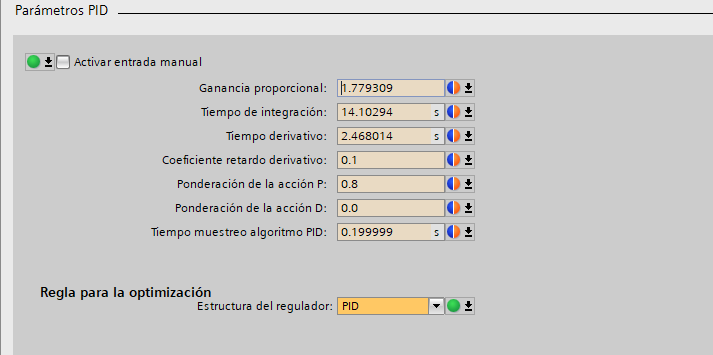
\includegraphics[width=0.9\textwidth]{images/proc_siemens_autotune_fc11.png}
        \caption{Resultado de la optimización inicial del controlador FC11 en TIA Portal.}
        \label{fig:proc_siemens_autotune_fc11}
    \end{figure}

    \item Convierta las siguientes variables a \textbf{DInt} y cree un \textbf{Trace} con ellas.
    \begin{itemize}
        \item FT10
        \item FT11
        \item Setpoint de FC11
        \item Esfuerzo de control de FC11
        \item Ratio deseado
        \item Ratio real
    \end{itemize}

    Se convirtieron las seis variables al tipo \textbf{DInt} y se configuró el \textbf{Trace} en TIA Portal para registrar su evolución temporal durante la prueba del control de ratio.

    \begin{figure}[H]
        \centering
        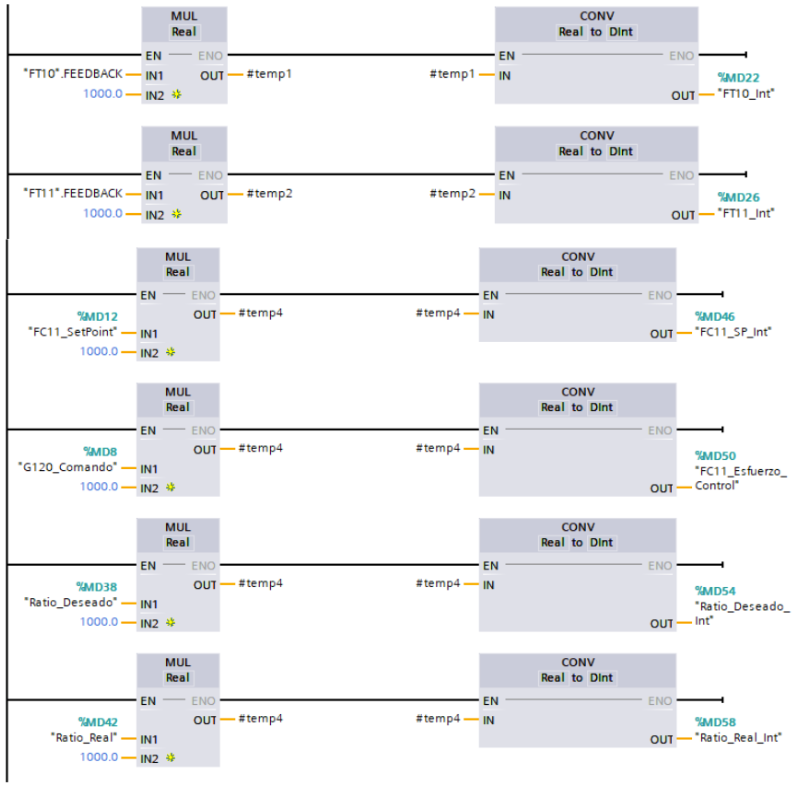
\includegraphics[width=0.9\textwidth]{images/proc_siemens_trace_config.png}
        \caption{Configuración del Trace en TIA Portal con las seis variables del control de ratio.}
        \label{fig:proc_siemens_trace_config}
    \end{figure}

  \begin{figure}[H]
        \centering
        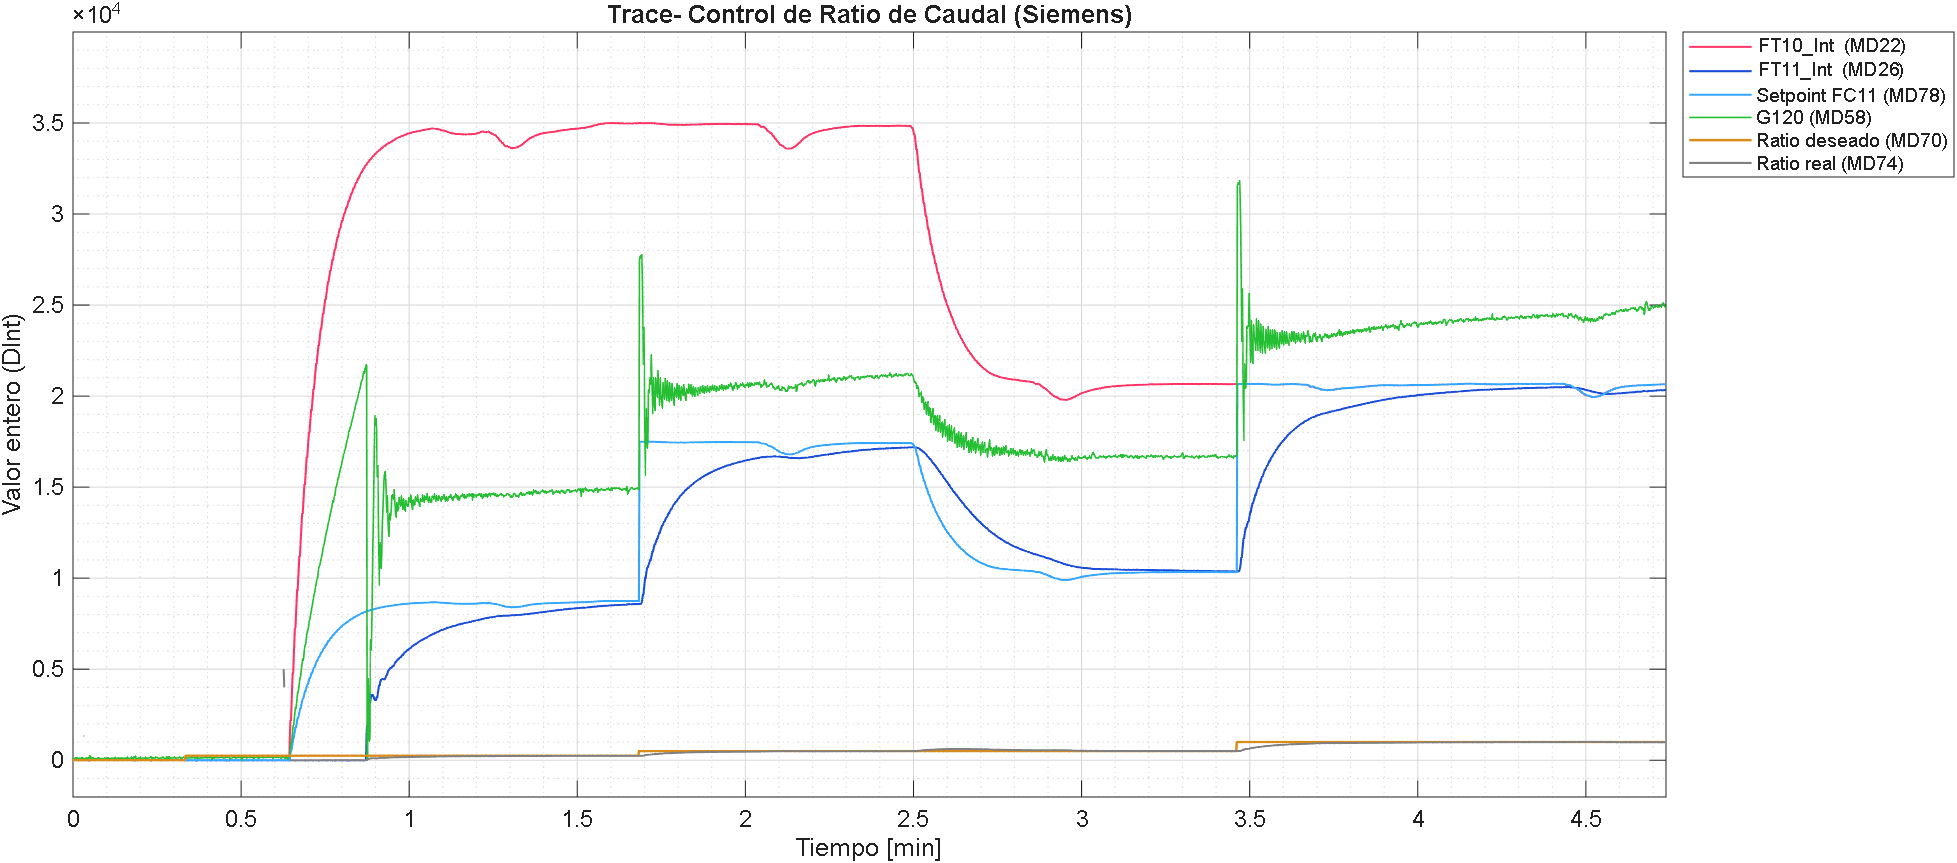
\includegraphics[width=0.9\textwidth]{images/proc_siemens_ratio_trace.png}
        \caption{Gráfica del Trace en TIA Portal con las seis variables del control de ratio.}
        \label{fig:proc_siemens_trace_config_trice}
    \end{figure}

    \item Realice el mismo procedimiento inicial que el item c). Establezca el caudal no controlado \textbf{FT10} abriendo la válvula \textbf{EV10}, y la válvula \textbf{EV11} al \textbf{40\%}. Cambie el \textbf{setpoint de FC11} al \textbf{setpoint de ratio} y pruebe el \textbf{control de ratio de caudal}. Mientras se ejecuta el control de ratio, abra la válvula \textbf{EV30}. Utilice \textbf{3 setpoints de ratio diferentes} dentro del rango que se muestra en el primer cuadro. Durante los dos últimos ratios, disminuya el porcentaje de apertura de la válvula \textbf{EV11} a \textbf{20\%} para cambiar el caudal medido por \textbf{FT10}. El \textbf{setpoint máximo} que se puede aplicar al controlador de caudal \textbf{FC11} se muestra en el segundo cuadro.

    \begin{center}
    \renewcommand{\arraystretch}{1.2}
    \begin{tabular}{|c|c|}
        \hline
        \textbf{Control de ratio de caudal} & \makecell[c]{\textbf{Setpoint de Ratio} \\ \textbf{(rango)}} \\\hline
        Prueba & 0.25 -- 1.25 \\\hline
    \end{tabular}
    \end{center}

    \begin{center}
    \renewcommand{\arraystretch}{1.2}
    \begin{tabular}{|c|}
        \hline
        \textbf{FC11 Setpoint máximo} \\\hline
        30 l/min \\\hline
    \end{tabular}
    \end{center}

    Se ejecutó la prueba del control de ratio con tres setpoints diferentes dentro del rango permitido (0.25--1.25). En el primer setpoint se mantuvo la válvula \textbf{EV11} al \textbf{40\,\%}, y durante los dos últimos se redujo la apertura al \textbf{20\,\%} para perturbar el caudal medido por FT10 y verificar la capacidad del lazo de ratio para mantener la relación deseada. El controlador FC11 ajustó automáticamente la velocidad del G120 para que el ratio real (FT11/FT10) siguiera al ratio deseado en cada caso.

    \begin{table}[H]
        \centering
        \renewcommand{\arraystretch}{1.2}
        \begin{tabular}{|c|c|c|}
            \hline
            \textbf{Prueba} & \textbf{Ratio deseado} & \textbf{Apertura EV11} \\ \hline
            1 & 0.4 & 40 \% \\ \hline
            2 & 0.6 & 20 \% \\ \hline
            3 & 0.8 & 20 \% \\ \hline
        \end{tabular}
        \caption{Valores de ratio deseado y apertura de EV11 utilizados durante la prueba.}
        \label{tab:proc_siemens_pruebas_ratio}
    \end{table}





    \item Utilizando los datos del \textbf{Trace} muestre los siguientes \textbf{gráficos}:
    \begin{itemize}
        \item Control de caudal FC11 -- Setpoint vs caudal medido
        \item Control de caudal FC11 -- Esfuerzo de control
        \item Ratio deseado vs medido
        \item FT10 vs FT11
    \end{itemize}

    Todas las figuras deben estar correctamente explicadas y tener leyenda, títulos, nombres de los labels y dimensiones correspondientes.

    A continuación se presentan los gráficos obtenidos a partir del Trace registrado durante la prueba del control de ratio.

    \begin{figure}[H]
        \centering
        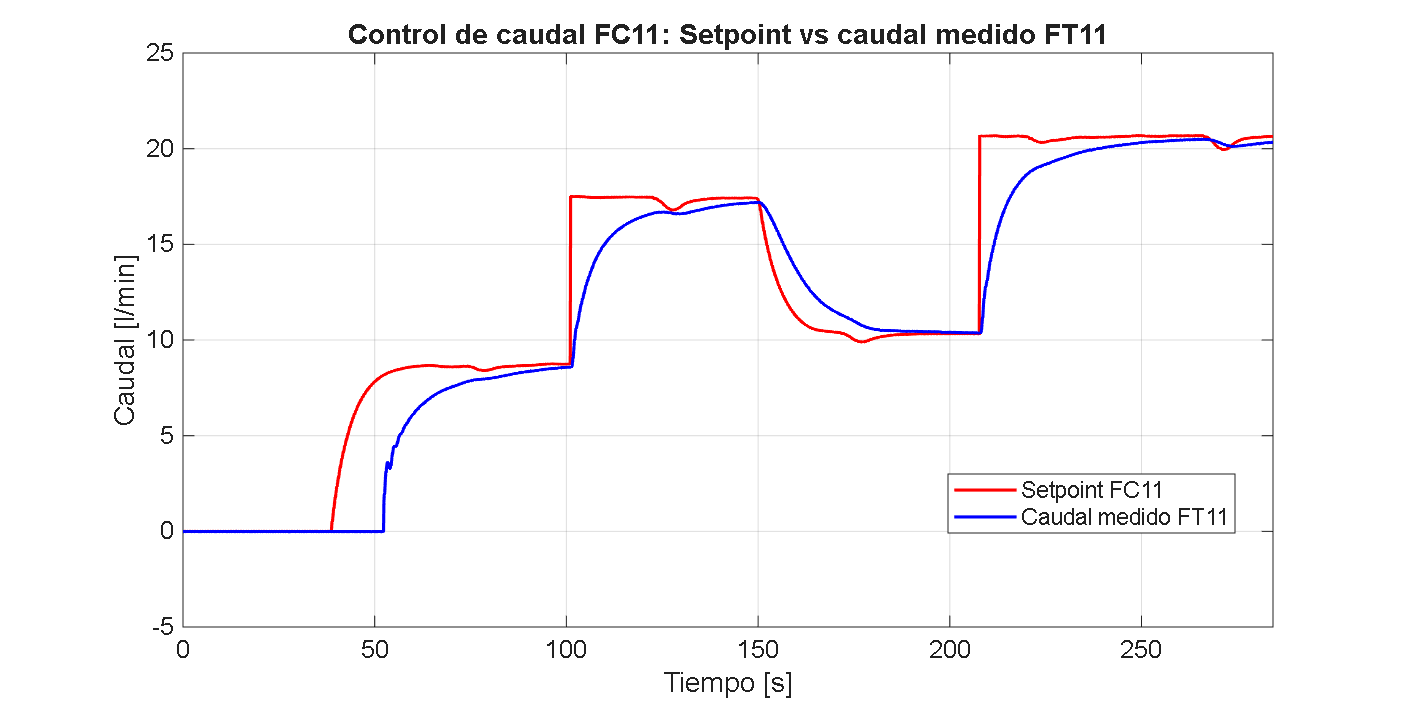
\includegraphics[width=0.95\textwidth]{images/proc_siemens_fc11_sp_vs_pv.png}
        \caption{Control de caudal FC11: setpoint (calculado como FT10 \(\times\) ratio) vs.\ caudal medido FT11.}
        \label{fig:proc_siemens_fc11_sp_vs_pv}
    \end{figure}

    \begin{figure}[H]
        \centering
        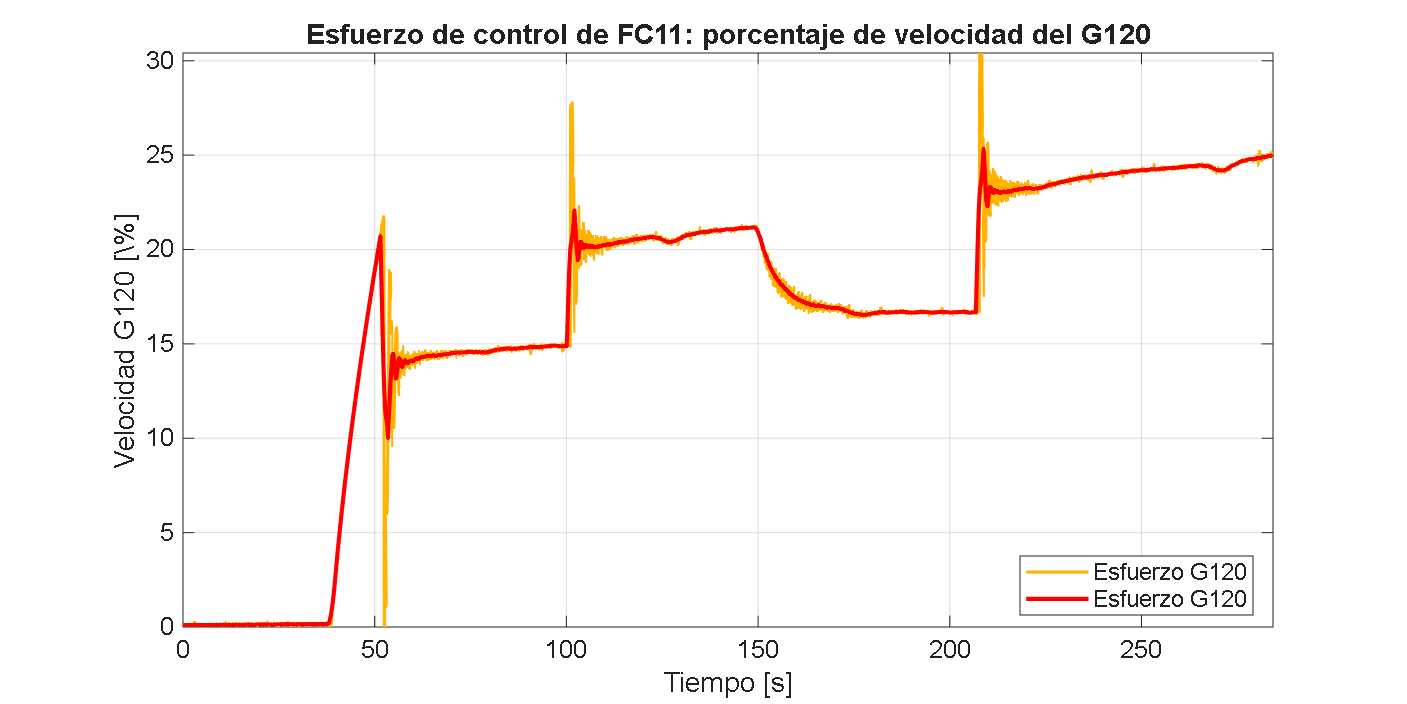
\includegraphics[width=0.95\textwidth]{images/proc_siemens_fc11_esfuerzo.png}
        \caption{Esfuerzo de control de FC11: porcentaje de velocidad comandado al G120.}
        \label{fig:proc_siemens_fc11_esfuerzo}
    \end{figure}

    \begin{figure}[H]
        \centering
        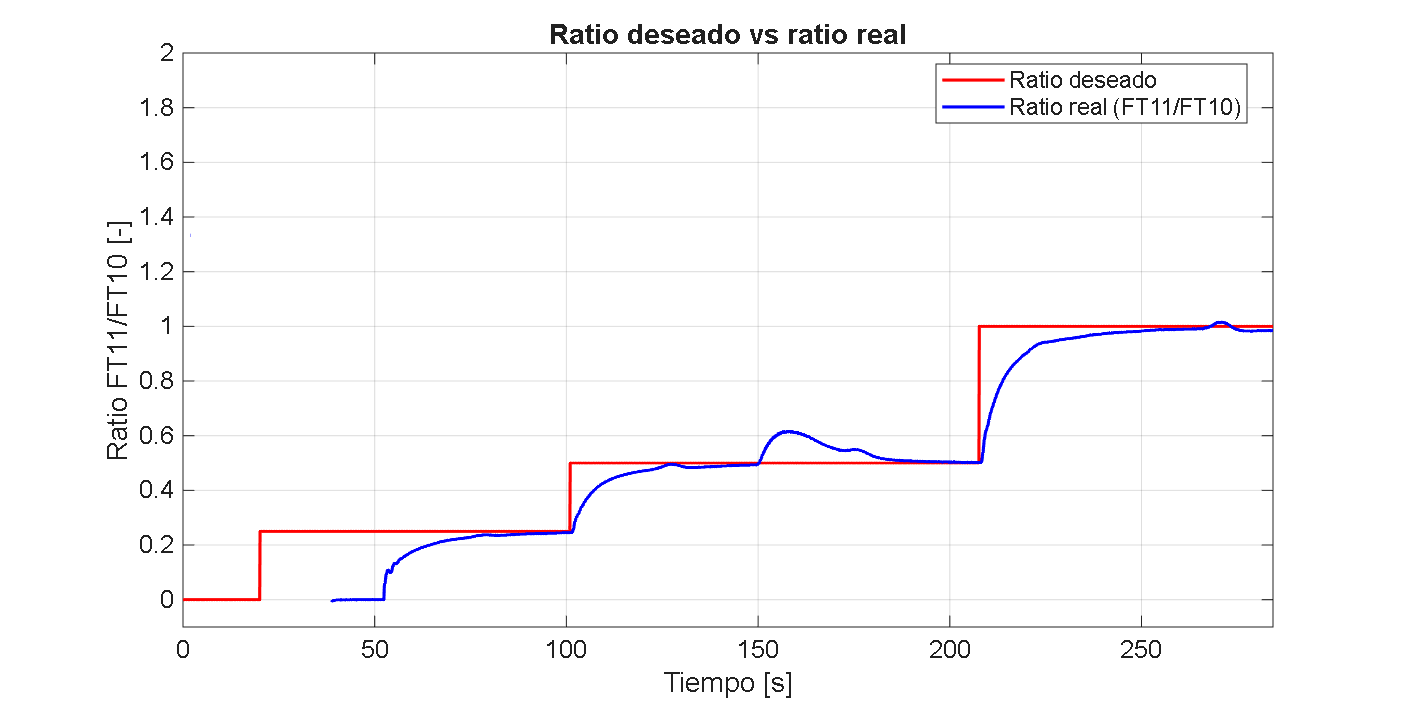
\includegraphics[width=0.95\textwidth]{images/proc_siemens_ratio_des_vs_med.png}
        \caption{Ratio deseado vs.\ ratio real (FT11/FT10) durante las tres pruebas.}
        \label{fig:proc_siemens_ratio_des_vs_med}
    \end{figure}

    \begin{figure}[H]
        \centering
        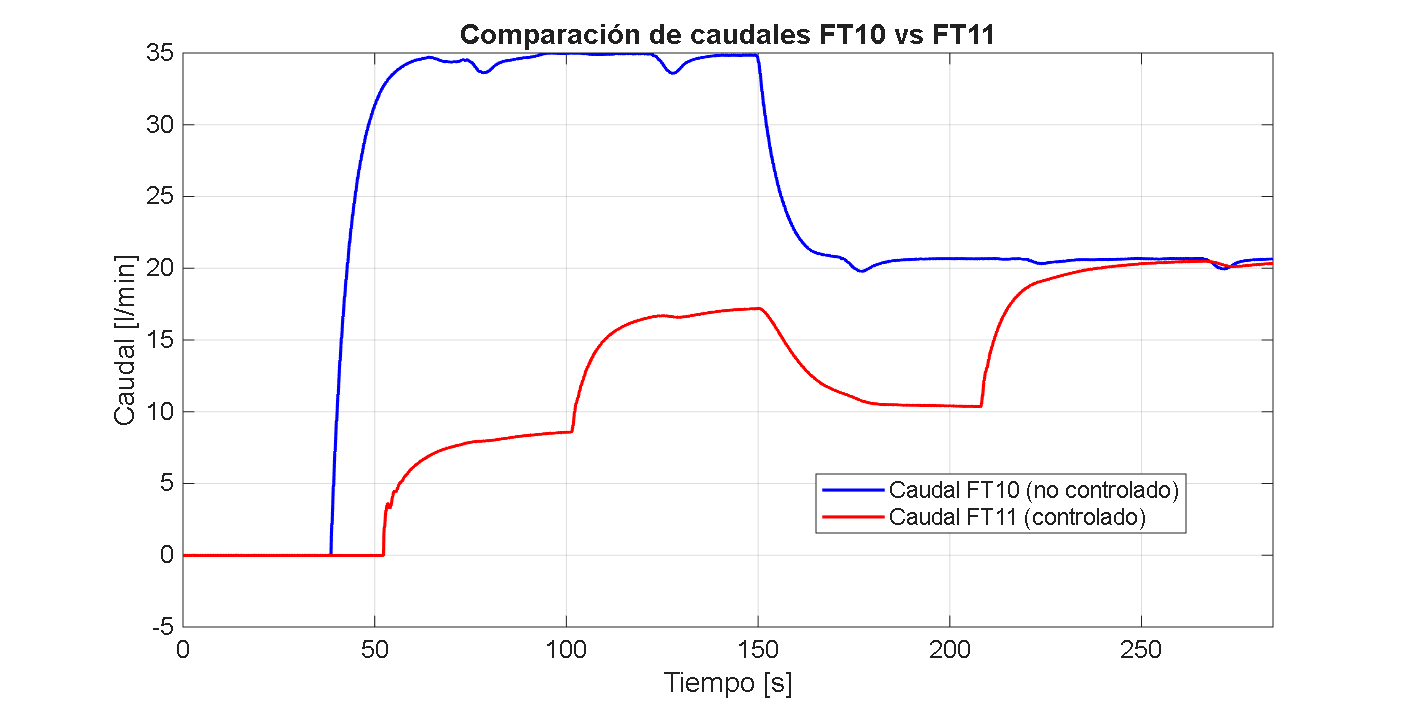
\includegraphics[width=0.95\textwidth]{images/proc_siemens_ft10_vs_ft11.png}
        \caption{Comparación de caudales FT10 y FT11 durante la prueba del control de ratio.}
        \label{fig:proc_siemens_ft10_vs_ft11}
    \end{figure}
\end{enumerate}






\subsubsection{Control en cascada de nivel a caudal}

\begin{enumerate}[label=\alph*)]
    \item Diseñe el \textbf{controlador de caudal secundario FC10} con la válvula \textbf{EV11} y el flujómetro \textbf{FT10} utilizando el bloque de instrucción \textbf{PID Compact} con la configuración que se muestra en la tabla. Cree todas las variables necesarias. Utilice un bloque \textbf{SEL} para cambiar entre un \textbf{setpoint de caudal manual} o de \textbf{cascada} para el controlador de caudal \textbf{FC10}.

    \begin{table}[H]
    \centering
    \renewcommand{\arraystretch}{1.2}
    \setlength{\tabcolsep}{5pt}
    \begin{tabular}{|>{\centering\arraybackslash}m{0.52\linewidth}|>{\centering\arraybackslash}m{0.24\linewidth}|}
    \hline
    \multicolumn{2}{|c|}{\textbf{PID FC10}} \\ \hline
    \textbf{Tipo de regulación} & Caudal (l/min) \\ \hline
    \textbf{Parámetros de entrada/salida} & \makecell[c]{Input: Input \\ Output: Output} \\ \hline
    \textbf{Limites del valor real} & 0.0 -- 80.0 l/min \\ \hline
    \textbf{Limites del valor de salida} & 0.0 -- 100 \% \\ \hline
    \end{tabular}
    \end{table}

    Se configuró el bloque \textbf{PID Compact} del controlador secundario FC10 con tipo de regulación \textit{Caudal (l/min)}, conectando como entrada la lectura del flujómetro FT10 y como salida el comando de apertura de la válvula EV11. Se añadió una instrucción \textbf{SEL} para alternar entre el setpoint manual y el setpoint proveniente del controlador primario LC10 (modo cascada).

    \begin{figure}[H]
        \centering
        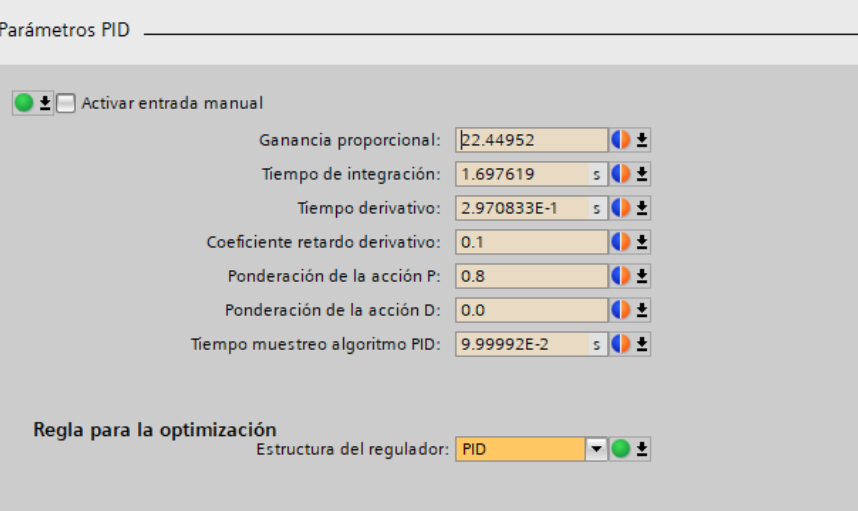
\includegraphics[width=0.85\textwidth]{images/proc_siemens_pid_fc10_config.png}
        \caption{Configuración del bloque PID Compact para el controlador secundario FC10 y el bloque SEL para selección de setpoint.}
        \label{fig:proc_siemens_pid_fc10_config}
    \end{figure}


    

    \item Diseñe el \textbf{controlador de nivel primario LC10} con el \textbf{setpoint de caudal FC10}, como salida y el sensor de nivel \textbf{PT10} utilizando una instrucción \textbf{PID Compact} con la configuración que se muestra en la tabla. Cree todas las variables necesarias.

    \begin{table}[H]
    \centering
    \renewcommand{\arraystretch}{1.2}
    \setlength{\tabcolsep}{5pt}
    \begin{tabular}{|>{\centering\arraybackslash}m{0.52\linewidth}|>{\centering\arraybackslash}m{0.24\linewidth}|}
    \hline
    \multicolumn{2}{|c|}{\textbf{PID LC10}} \\ \hline
    \textbf{Tipo de regulación} & General (\%) \\ \hline
    \textbf{Limites del valor real} & 0.0 -- 100.0 \% \\ \hline
    \textbf{Limites del valor de salida} & 0.0 -- 30.0 \% \\ \hline
    \end{tabular}
    \end{table}

    Se configuró el bloque \textbf{PID Compact} del controlador primario LC10 con tipo de regulación \textit{General (\%)}, conectando como entrada la lectura del sensor de nivel PT10 y como salida el setpoint del controlador secundario FC10. Los límites de la salida (0--30\,\%) corresponden a la fracción del rango de caudal permitido en modo cascada.

    \begin{figure}[H]
        \centering
        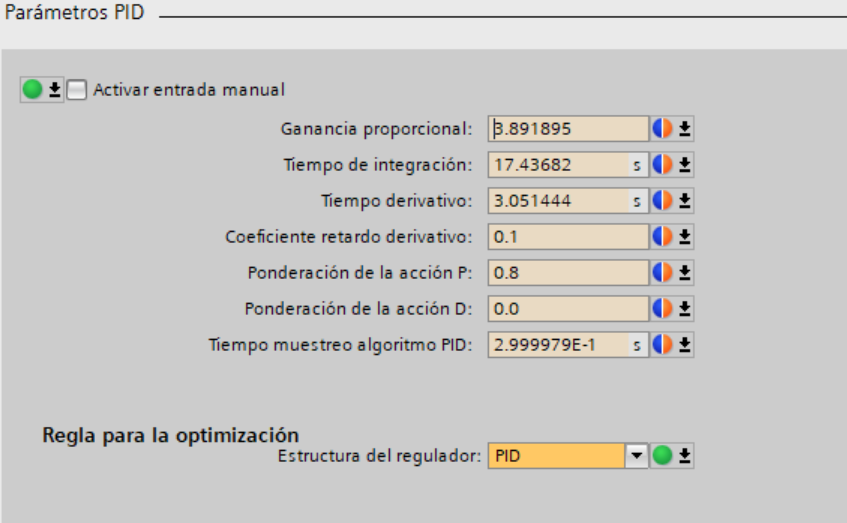
\includegraphics[width=0.85\textwidth]{images/proc_siemens_pid_lc10_config.png}
        \caption{Configuración del bloque PID Compact para el controlador primario LC10 (lazo de nivel).}
        \label{fig:proc_siemens_pid_lc10_config}
    \end{figure}

    \item Abra la válvula \textbf{EV10} y \textbf{autosintonice el controlador secundario} diseñado mediante la opción ``\textbf{Optimización inicial}'' con el \textbf{Setpoint} que se muestra en la tabla. Asegúrese de que la \textbf{válvula de desfogue manual} del tanque superior esté \textbf{abierta}, de manera que el tanque superior no se llene y no se active el \textbf{interlock de seguridad}. Después de la optimización, mostrar las \textbf{ganancias PID} obtenidas.

    \begin{center}
    \renewcommand{\arraystretch}{1.2}
    \begin{tabular}{|c|c|}
        \hline
        \textbf{FC10} & \textbf{Setpoint} \\\hline
        Optimización & 30 l/min \\\hline
    \end{tabular}
    \end{center}

    Tras abrir la válvula EV10 y la válvula de desfogue manual del tanque superior, se ejecutó la \textit{Optimización inicial} del controlador secundario FC10 con un setpoint de \textbf{30 l/min}. Las ganancias PID obtenidas se muestran en la Tabla~\ref{tab:proc_siemens_gains_fc10}.

    \begin{table}[H]
        \centering
        \renewcommand{\arraystretch}{1.2}
        \begin{tabular}{|l|c|}
            \hline
            \textbf{Parámetro} & \textbf{Valor obtenido} \\ \hline
            \(K_p\) (Ganancia proporcional) &  27.16934\\ \hline
            \(T_i\) (Tiempo integral) &  1.321296 s\\ \hline
            \(T_d\) (Tiempo derivativo) &  0.2312268 s\\ \hline
        \end{tabular}
        \caption{Ganancias PID del controlador secundario FC10 obtenidas mediante optimización inicial.}
        \label{tab:proc_siemens_gains_fc10}
    \end{table}

    \begin{figure}[H]
        \centering
        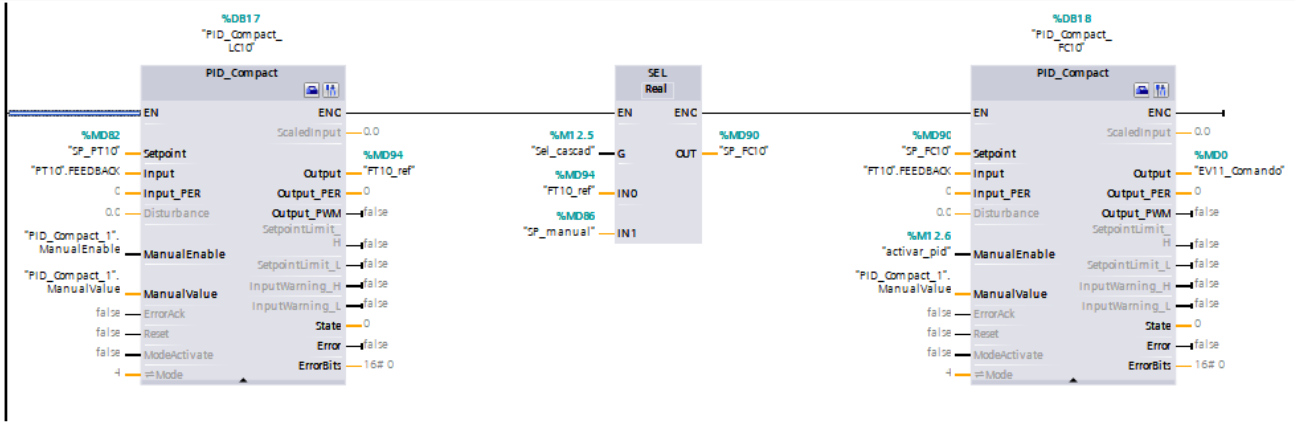
\includegraphics[width=0.9\textwidth]{images/proc_siemens_autotune_fc10.png}
        \caption{Resultado de la optimización inicial del controlador secundario FC10 en TIA Portal.}
        \label{fig:proc_siemens_autotune_fc10}
    \end{figure}

    \item Abra la válvula \textbf{EV10}, configure el controlador de caudal \textbf{FC10} en \textbf{Auto} y \textbf{autosintonice} el controlador primario diseñado mediante la opción ``\textbf{Optimización inicial}'' con el \textbf{Setpoint} que se muestra en la tabla. Asegúrese de que la válvula \textbf{DV30} y la \textbf{válvula de desfogue manual} del tanque superior estén \textbf{cerradas}. Después de la optimización, muestre las \textbf{ganancias PID} obtenidas.

    \begin{center}
    \renewcommand{\arraystretch}{1.2}
    \begin{tabular}{|c|c|}
        \hline
        \textbf{LC10} & \textbf{Setpoint} \\\hline
        Optimización & 50 \% \\\hline
    \end{tabular}
    \end{center}

    Con el lazo interno (FC10) en modo \textbf{Auto} y las válvulas DV30 y de desfogue manual cerradas, se ejecutó la \textit{Optimización inicial} del controlador primario LC10 con un setpoint de nivel de \textbf{50\,\%}. Las ganancias PID obtenidas se muestran en la Tabla~\ref{tab:proc_siemens_gains_lc10}.

    \begin{table}[H]
        \centering
        \renewcommand{\arraystretch}{1.2}
        \begin{tabular}{|l|c|}
            \hline
            \textbf{Parámetro} & \textbf{Valor obtenido} \\ \hline
            \(K_p\) (Ganancia proporcional) &  3.723639\\ \hline
            \(T_i\) (Tiempo integral) &  17.86652 s\\ \hline
            \(T_d\) (Tiempo derivativo) &  3.12664 s\\ \hline
        \end{tabular}
        \caption{Ganancias PID del controlador primario LC10 obtenidas mediante optimización inicial.}
        \label{tab:proc_siemens_gains_lc10}
    \end{table}

    \begin{figure}[H]
        \centering
        \includegraphics[width=0.9\textwidth]{images/proc_siemens_autotune_lc10.png}
        \caption{Resultado de la optimización inicial del controlador primario LC10 en TIA Portal.}
        \label{fig:proc_siemens_autotune_lc10}
    \end{figure}

    \item Convierta las siguientes variables a \textbf{DInt} y cree un \textbf{Trace} con ellas.
    \begin{itemize}
        \item FT10
        \item Setpoint de FC10
        \item Esfuerzo de control de FC10
        \item PT10
        \item Setpoint de LC10
    \end{itemize}

    Se convirtieron las cinco variables al tipo \textbf{DInt} y se configuró el \textbf{Trace} en TIA Portal para registrar la evolución temporal del lazo en cascada durante la prueba.

    \begin{figure}[H]
        \centering
        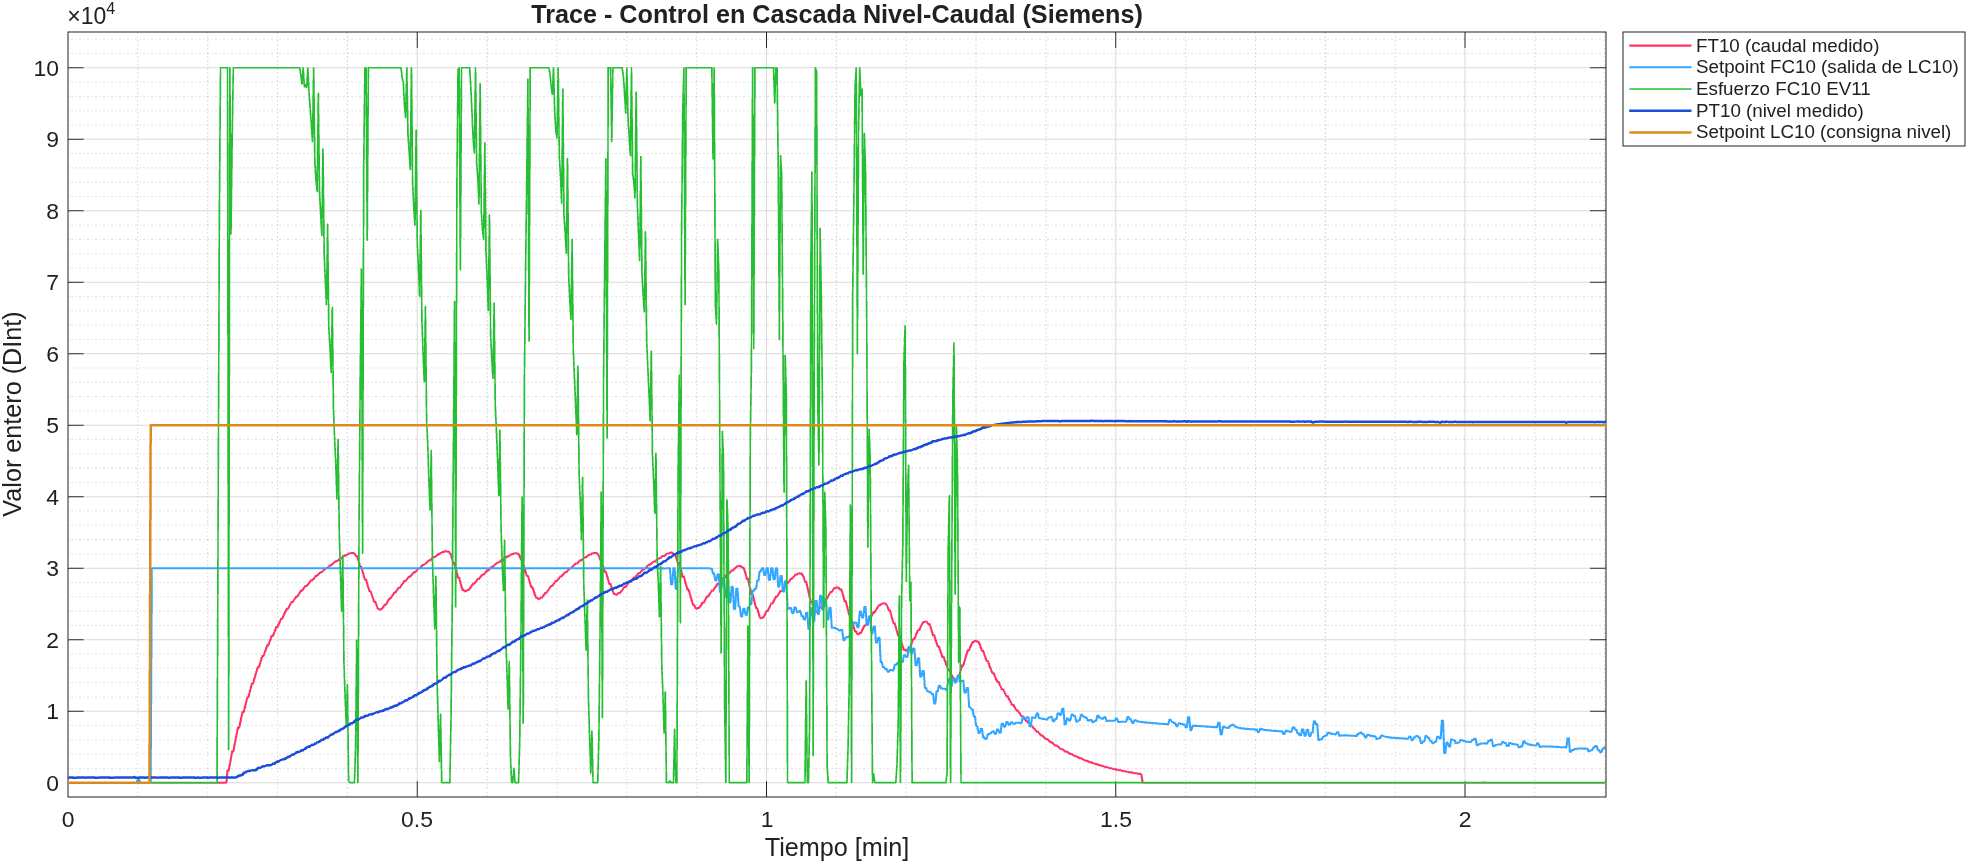
\includegraphics[width=0.9\textwidth]{images/proc_siemens_cascada_trace.png}
        \caption{Configuración del Trace en TIA Portal con las cinco variables del control en cascada.}
        \label{fig:proc_siemens_trace_cascada_config}
    \end{figure}

    \item[h)] Configure el controlador de caudal \textbf{FC10} y el controlador de nivel \textbf{LC10} en modo \textbf{Auto}. Pruebe el control en cascada de nivel a caudal con un \textbf{setpoint} dentro del rango que se muestra en la tabla. Mientras realiza el control en cascada de nivel a caudal, asegúrese de que la válvula \textbf{DV30} y la \textbf{válvula de desfogue manual} del tanque superior estén \textbf{cerradas}.

    \begin{center}
    \renewcommand{\arraystretch}{1.2}
    \begin{tabular}{|c|c|}
        \hline
        \textbf{PID LC10} & \makecell[c]{\textbf{Setpoint de nivel} \\ \textbf{(rango)}} \\\hline
        Prueba & 25-85 \% \\\hline
    \end{tabular}
    \end{center}

    Con ambos controladores en modo \textbf{Auto} y las válvulas DV30 y de desfogue manual cerradas, se probó el control en cascada de nivel a caudal aplicando un setpoint de nivel dentro del rango 25--85\,\%. El lazo primario LC10 calculó el setpoint de caudal requerido, el cual fue seguido por el lazo secundario FC10 mediante la manipulación de la apertura de la válvula EV11.

    \item Utilizando los datos del \textbf{Trace} muestre los siguientes \textbf{gráficos}:
    \begin{itemize}
        \item Control de caudal FC10 -- Setpoint vs caudal medido
        \item Control de caudal FC10 -- Esfuerzo de control
        \item Control en cascada de nivel a caudal LC10: Setpoint vs nivel medido
    \end{itemize}

    Todas las figuras deben estar correctamente explicadas y tener leyenda, títulos, nombres de los labels y dimensiones.

    A continuación se presentan los gráficos obtenidos del Trace registrado durante la prueba del control en cascada.

    \begin{figure}[H]
        \centering
        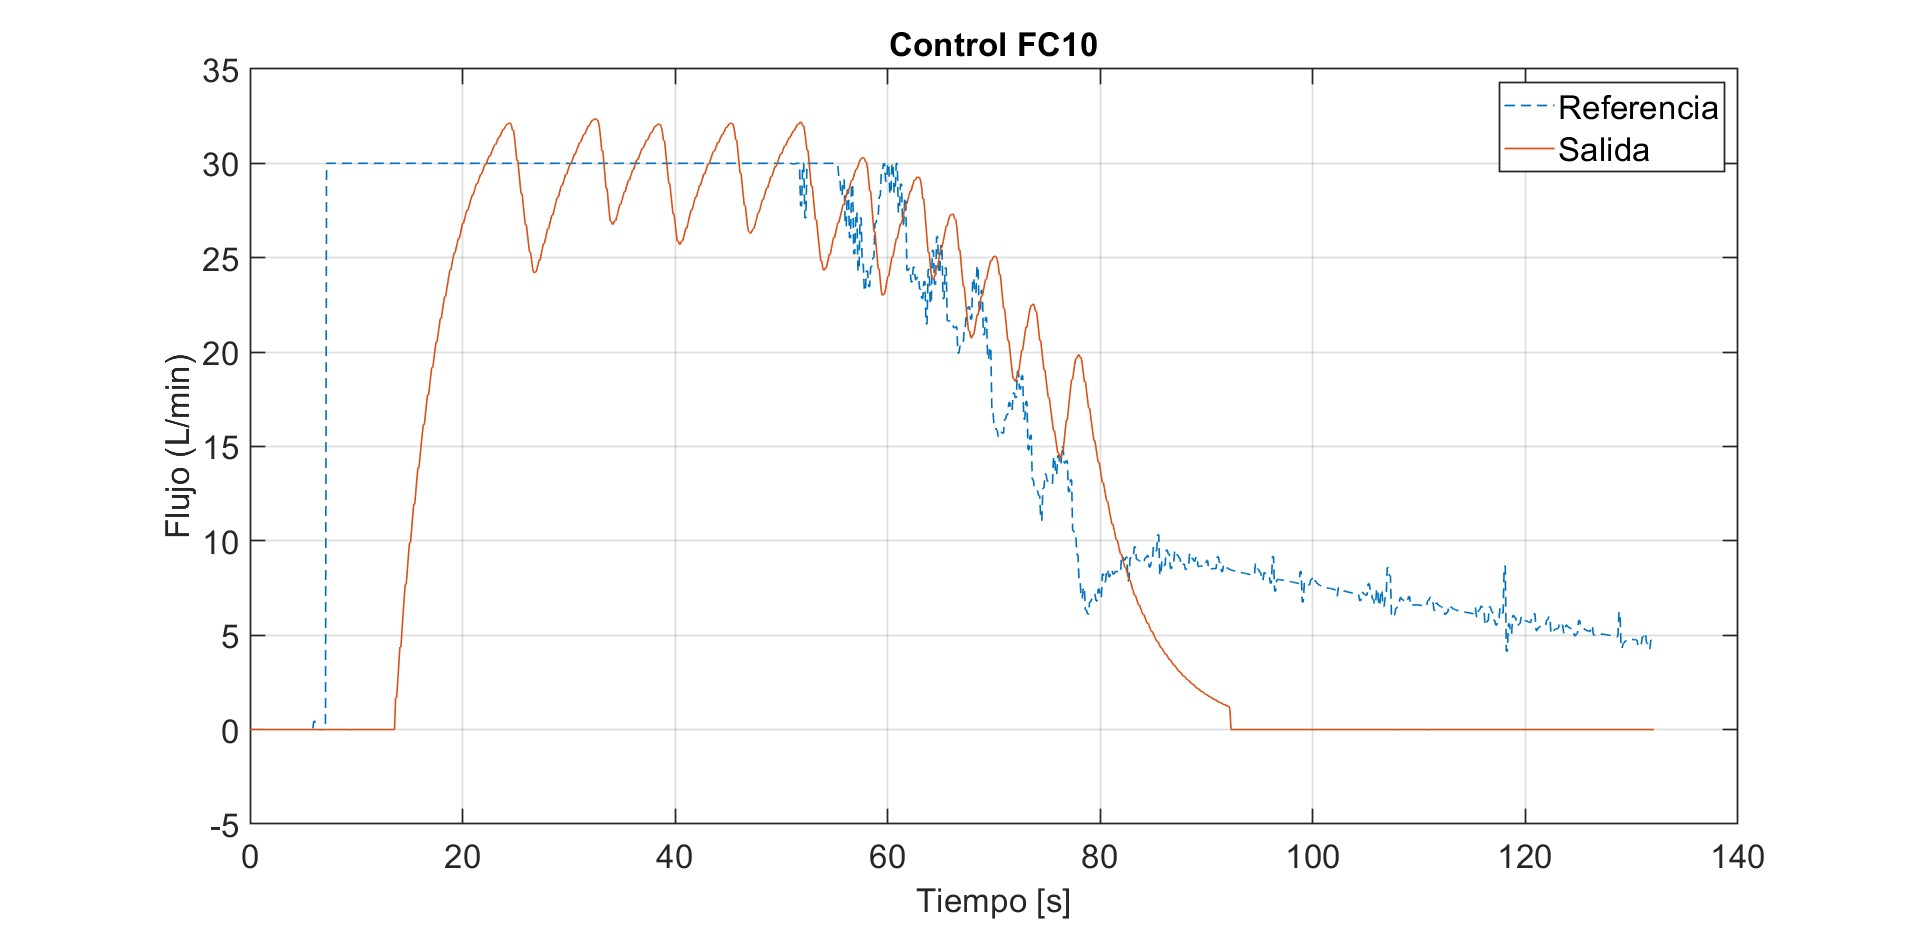
\includegraphics[width=0.95\textwidth]{images/control_fc10.jpg}
        \caption{Control de caudal FC10: setpoint (generado por LC10) vs.\ caudal medido FT10.}
        \label{fig:proc_siemens_fc10_sp_vs_pv}
    \end{figure}

    \begin{figure}[H]
        \centering
        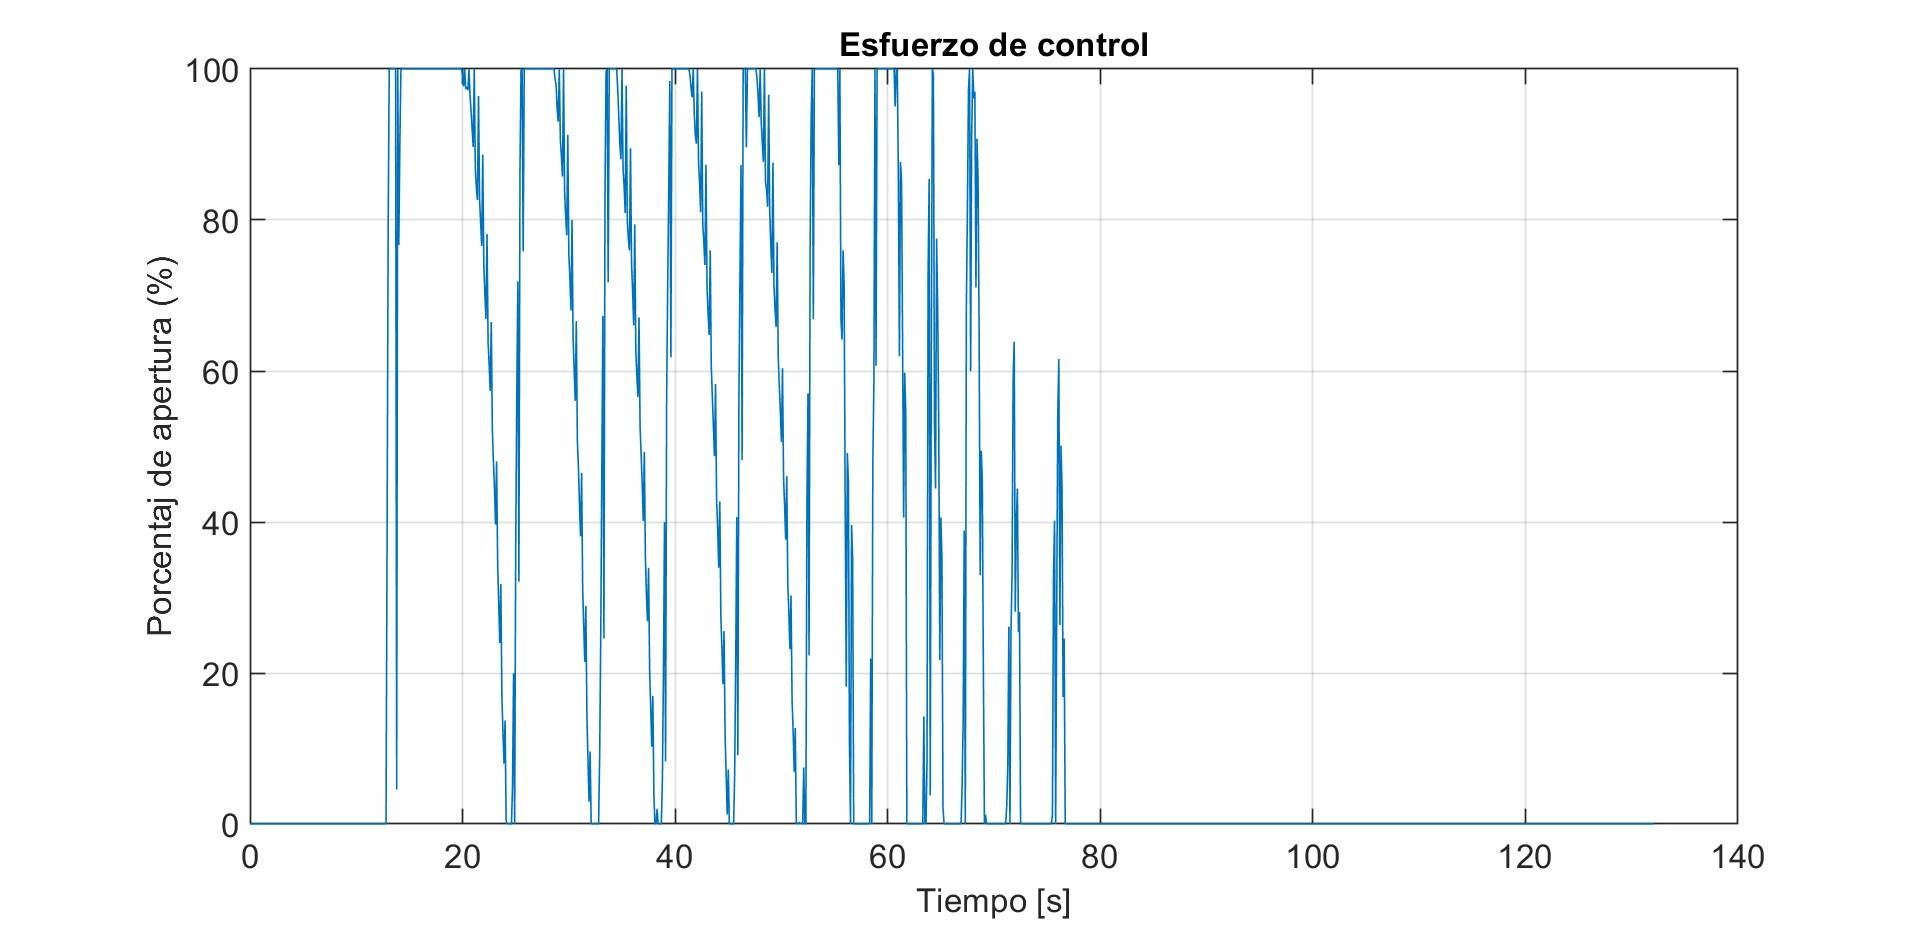
\includegraphics[width=0.95\textwidth]{images/esfuerzo_de_Control.jpg}
        \caption{Esfuerzo de control de FC10: porcentaje de apertura de la válvula EV11.}
        \label{fig:proc_siemens_fc10_esfuerzo}
    \end{figure}

    \begin{figure}[H]
        \centering
        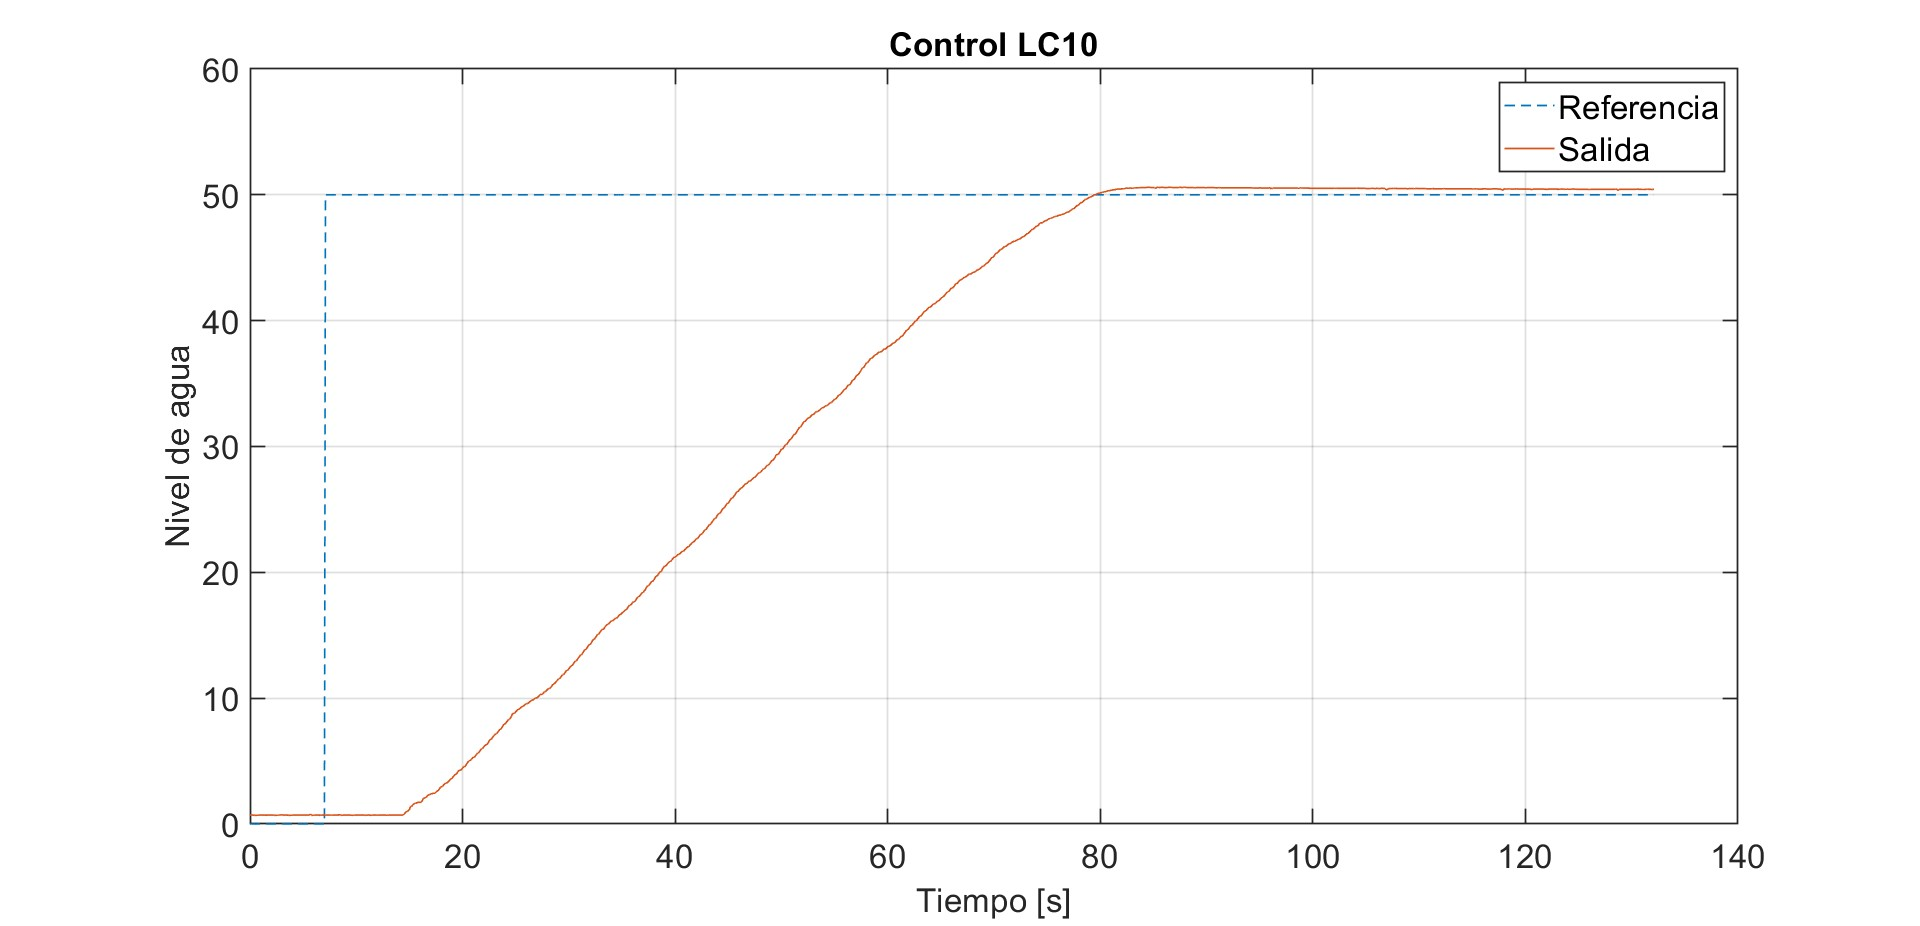
\includegraphics[width=0.95\textwidth]{images/control_lc10.jpg}
        \caption{Control en cascada LC10: setpoint de nivel vs.\ nivel medido en el tanque T-10 (PT10).}
        \label{fig:proc_siemens_lc10_sp_vs_pv}
    \end{figure}

    \item[\textbf{Reto.}] Añada una \textbf{lógica} para evitar que siga ingresando caudal al tanque T-10 una vez que el nivel real se encuentre dentro de un rango aceptable alrededor del \textbf{setpoint de nivel}. Esta lógica es necesaria debido a que, aunque la salida del controlador primario \textbf{LC10} sea cercana o igual a \textbf{0 l/min}, el bloque \textbf{PID Compact} del controlador secundario \textbf{FC10} puede seguir enviando un pequeño comando a la válvula \textbf{EV11}, lo cual ocasiona que, en un tiempo prolongado, el nivel del tanque aumente lentamente. Explique la lógica implementada.

    Se implementó una \textbf{lógica de banda muerta} alrededor del setpoint de nivel: cuando el valor absoluto del error \(|SP_{nivel} - PT10|\) es menor a un umbral definido (por ejemplo, \(\pm 2\,\%\)), una compuerta lógica fuerza la salida hacia la válvula EV11 a \textbf{0\,\%}, anulando el comando residual del PID Compact del FC10. Cuando el error sale del rango aceptable, la lógica devuelve el control a la salida normal del FC10. Esto evita el llenado lento del tanque por el comando residual del lazo secundario.

    \begin{figure}[H]
        \centering
        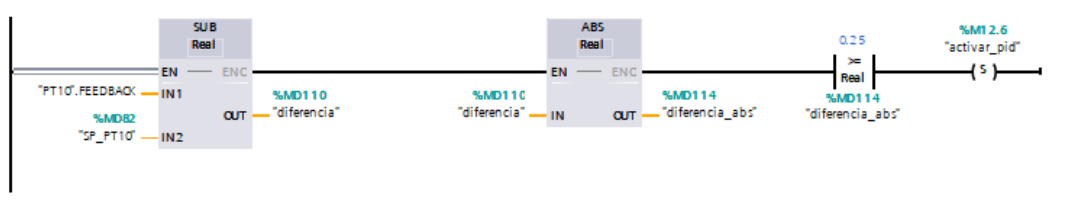
\includegraphics[width=0.95\textwidth]{images/proc_siemens_logica_reto.png}
        \caption{Lógica implementada para anular el comando residual de FC10 cuando el nivel está dentro del rango aceptable del setpoint.}
        \label{fig:proc_siemens_logica_reto}
    \end{figure}

\end{enumerate}